\section{Приложение Тест (Задание 9)}

\subsection{Условие задания}

Создать приложение для проведения тестирования.

Должно содержать:


\begin{enumerate}
    \item{Набор вопросов по какой"=то теме (и вопросы и ответы должны быть реальные) --- не менее 10}
    \item{Вопросы должны выбираться случайным образом.}
    \item{Вопросы должны быть нескольких типов --- "Да/нет", Выбор одного ответа, Выбор нескольких ответов, Короткий ответ.}
    \item{Необходимо создать сообщения для правильного и неправильного ответа (Молодец, Не правильно и т.д.)}
    \item{Необходимо подсчитать количество правильных ответов и вывести результат.}
\end{enumerate}

\subsection{Вид формы в конструкторе}

Форма имеет вид (рис.\ref{fig:FormInConstruct9}):

\begin{figure}[!h]
    \centering
    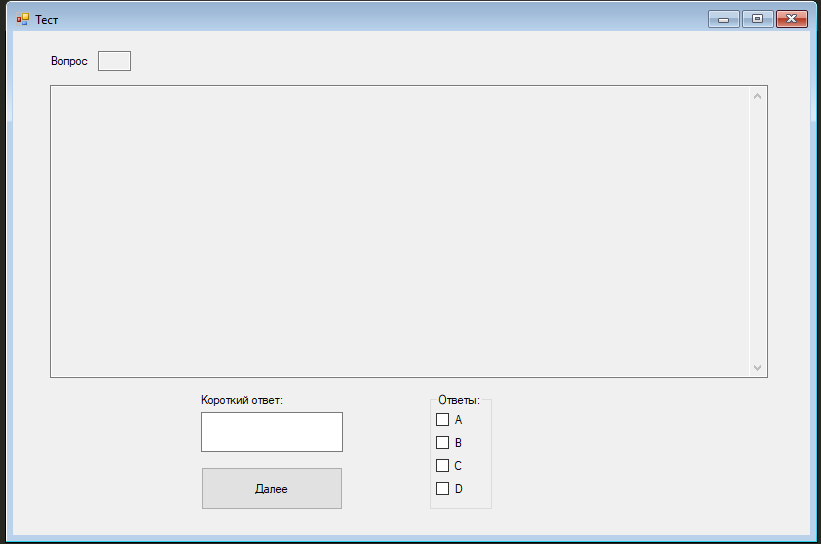
\includegraphics[width = 0.75\textwidth]{images/Task9/FormInConstructor.png}
    \caption{Вид формы в конструкторе}
    \label{fig:FormInConstruct9}
\end{figure}

\subsection{Таблица с описанием переименовнных элементов формы}

Все элементы формы были переименованы и их атрибыты изменены. Проведенные изменения представлены в таблице \ref{tab:label9}

\begin{longtable}[!h]{|l|l|l|}
    \caption{Значения атрибутов элементов в приложении <<Тест>>}
    \label{tab:label9}
    \endfirsthead
    \endhead
    \hline
    \makecell{$\textbf{Описание элементов}$\\ $\textbf{формы}$}& \makecell{$\textbf{Список измененных}$\\ $\textbf{атрибутов}$}& \makecell{$\textbf{Новое значение}$\\ $\textbf{атрибута}$}\\ 
    \hline
    \makecell{Форма}& \makecell{Text}& \makecell{Тест}\\ 
    \hline
    \makecell{Первая надпись (label)}& \makecell{Name}& \makecell{lblQuest}\\ 
    \hline
    \makecell{Первая надпись (label)}& \makecell{Text}& \makecell{Вопрос:}\\ 
    \hline
    \makecell{Вторая надпись (label)}& \makecell{Name}& \makecell{lblShortAnswer}\\ 
    \hline
    \makecell{Вторая надпись (label)}& \makecell{Text}& \makecell{Короткий ответ:}\\ 
    \hline

    \makecell{Кнопка (button)}& \makecell{Name}& \makecell{actionBtn}\\ 
    \hline
    \makecell{Кнопка (button)}& \makecell{Text}& \makecell{Далее}\\ 
    \hline

    \makecell{Первое текстовое\\ поле (textBox)}& \makecell{Name}& \makecell{countBox}\\ 
    \hline
    \makecell{Первое текстовое\\ поле (textBox)}& \makecell{ReadOnly}& \makecell{True}\\ 
    \hline
    \makecell{Второе текстовое\\ поле (textBox)}& \makecell{Name}& \makecell{questBox}\\ 
    \hline
    \makecell{Второе текстовое\\ поле (textBox)}& \makecell{ReadOnly}& \makecell{True}\\ 
    \hline
    \makecell{Третье текстовое\\ поле (textBox)}& \makecell{Name}& \makecell{shortAnswerBox}\\ 
    \hline

    \makecell{groupBox}& \makecell{Name}& \makecell{answerGroup}\\ 
    \hline

    \makecell{checkBox}& \makecell{Name}& \makecell{answerA}\\ 
    \hline
    \makecell{checkBox}& \makecell{Name}& \makecell{answerB}\\ 
    \hline
    \makecell{checkBox}& \makecell{Name}& \makecell{answerC}\\ 
    \hline
    \makecell{checkBox}& \makecell{Name}& \makecell{answerD}\\ 
    \hline

    \makecell{Обработчик ошибок\\ (errorProvider)}& \makecell{Name}& \makecell{errPr}\\ 
    \hline
\end{longtable}

\subsection{Примеры работы}

При запуске приложения на экране появляется окно с одним из случайно выбранных вопросов (рис.\ref{fig:StartForm9}).

\newpage

\begin{figure}[!h]
    \centering
    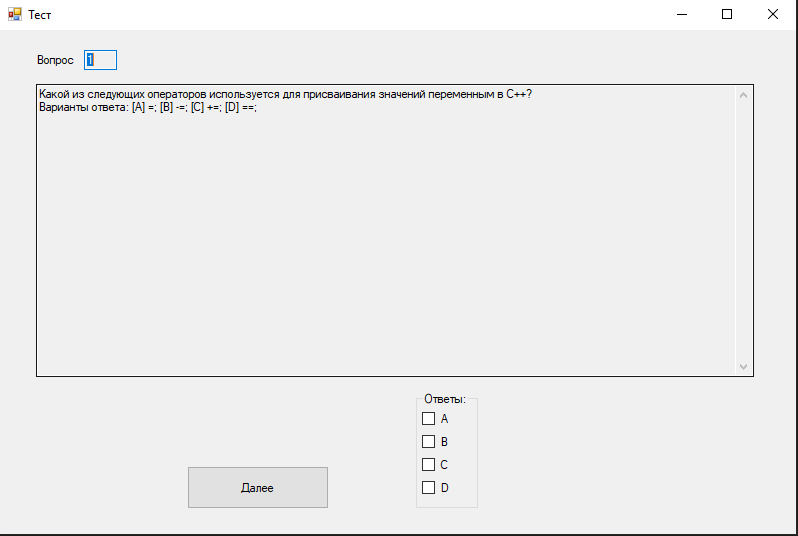
\includegraphics[width = 0.7\textwidth]{images/Task9/OneAnswer.png}
    \caption{Запуск приложения}
    \label{fig:StartForm9}
\end{figure}

При запуске с корректными данными (правильным ответом в данном примере), при нажатии на кнопку <<Далее>> происходит (рис.\ref{fig:WorkForm9}):

\begin{figure}[!h]
    \centering
    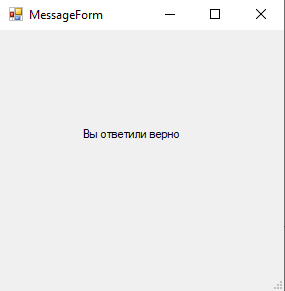
\includegraphics[width = 0.4\textwidth]{images/Task9/RightAnswer.png}
    \caption{Запуск с корректными данными}
    \label{fig:WorkForm9}
\end{figure}

При запуске с некорректными данными, при нажатии на кнопку <<Далее>> происходит (рис.\ref{fig:BadInputNotIntForm9}):

\newpage

\begin{figure}[!h]
    \centering
    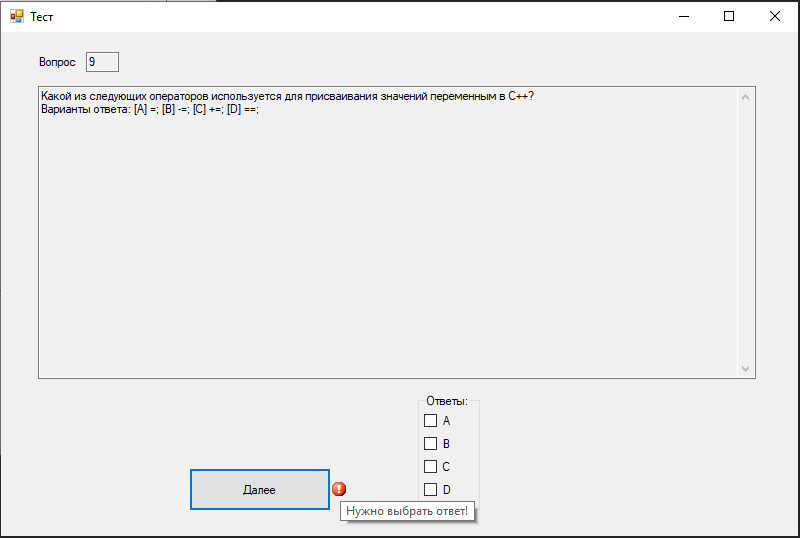
\includegraphics[width = 0.8\textwidth]{images/Task9/OneAnswerBadInput.png}
    \caption{Запуск с некорректными данными}
    \label{fig:BadInputNotIntForm9}
\end{figure}

\subsection{Примеры кода}

Функция отображения в зависимости от вопроса нужных элементов на форме:

\begin{minted}{c++}
		// Функция выбора формы
		void ChooseForm() {
			int i = RandIndex->at(iter);
			Quest temp = Questions->at(i);
			// В зависимости от вопроса вызываем нужную функцию отображения элементов на форме
			if (temp.getType() == YesNo) {
				YesNoForm();
			}
			else if (temp.getType() == OneAnswer || temp.getType() == SomeAnswers) {
				OneAnswerForm();
			}
			else {
				ShortAnswerForm();
			}
		}
\end{minted}

Другие фрагменты кода расположены в приложении \ref{app:task9}. Полный код программы приведен в приложении \ref{app:zip}
